\documentclass{article}

\usepackage[utf8]{inputenc}
\usepackage{mathtools}             % For symbols like tilde
\usepackage[T1]{fontenc}           % For symbols like tilde
\usepackage{hyperref}              % For \url{...}
\usepackage{amssymb}               % Math symbols
\usepackage{amsmath}               % Various commands like \text{...}
\usepackage{mathtools}             % Maths
\usepackage[noend]{algpseudocode}  % Pseudocode printer
\usepackage{listings}              % Source code printer
\usepackage{framed}                % To frame the computational cost
\usepackage{qtree}                 % Draw simple binary trees
\usepackage{amsthm}                % \proof environment
\usepackage{titlesec}              % Customize sections

\newcommand*{\expect}[1]{\mathsf{E}\left[{#1}\right]} % Define statistical expected value
\newcommand*{\prob}{\mathsf{P}}                       % Define statistical probability
\newcommand{\sectionbreak}{\clearpage}                % Clear page before each section

\DeclarePairedDelimiter\abs{\lvert}{\rvert}           % Define abs-like syntax
\DeclarePairedDelimiter\norm{\lVert}{\rVert}
\DeclareMathOperator*{\median}{median}                % Median operator

\lstset{numbers=left} % Print line numbers in \begin{lstlisting}...

\title{Advanced Algorithms Problems and Solutions}
\author{Mattia Setzu \and Giorgio Vinciguerra}
\date{October 2016}

\begin{document}

  \maketitle
  \tableofcontents

  \section{Range updates}

Consider an array $C$ of $n$ integers, initially all equal to zero. We want to support the following operations:
\begin{itemize}
  \item $update(i, j, c)$, where $0 \leq i \leq j \leq n - 1$ and $c$ is an integer: it changes $C$ such that $C[k] := C[k] + c$ for every $i \leq k \leq j$.
  \item $query(i)$, where $0 \leq i \leq n - 1$: it returns the value of $C[i]$.
  \item $sum(i,j)$, where $0 \leq i \leq j \leq n - 1$: it returns $\sum_{k = 1}^j C[k]$.
\end{itemize}

Design a data structure that uses $O(n)$ space, takes $O(n \log n)$ construction time, and implements each operation above in $O(\log n)$ time. Note that $query(i) = sum(i, i)$ but it helps to reason.

[Hint: For the general case, use the segment tree seen in class, which uses $O(n \log n)$ space: prove that its space is actually $O(n)$ when it is employed for this problem.]

\subsection{First solution}

Let $T$ be a segmented binary tree over a continuous interval $I: [0, N - 1]$
s.t.\ its leafs are the points in I, and the parent of two nodes comprises of their interval:
$$  n' \cup n'' = n, n' \cap n'' = \emptyset   \textrm{ s.t. } n \text{ is the parent of } n', n''$$

$T$ will keep track of the prefix sums for every interval.
We define a function
\begin{equation}
    s': [0, n - 1] \to \mathbb{N}
\end{equation}
that given a node in $T$ returns the value associated with $I$, namely the
cumulative sum of that interval.

In order to reduce the computational cost, we introduce a lazy algorithm
that doesn't propagate sums over $T$ as they are streamed in the input,
which means $s'(i)$ might not be accurate at a given time $t$ for any of the
requested operation.

We'll instead either compute over $T$ or update $T$ as necessary.
Let us define a function to do so:
\begin{equation}
    l: \mathbb{N} \to (\mathbb{N} \cup \{\epsilon\}, \mathbb{N})
\end{equation}
to keep track of our lazy sums:
\begin{equation}
    s(n) = \begin{cases}
            \epsilon, \_            &   \textrm{if no lazy prefix sum is in that interval} \\
            k, m                    &   \textrm{if a lazy sum of k is to be propagated to m}\\
            \end{cases}
\end{equation}
The \textsc{query} function is then trivial:

\begin{algorithmic}[1]
    \Function{query}{$I$, $i$, $sum$}:
    \If{$I.size = 1$}                       \Comment{Return found value}
      \State \Return $I.sum$
    \EndIf
    \If{lazy(I), $i \in I.left, i \notin I.right$}     \Comment{Lazy on left child}
      \State $lazy(I) \gets False$
      \State \Call{query}{$I.left$, $i$, $sum + I.sum$}
    \EndIf
    \If{lazy(I), $i \in I.right, i \notin I.left$} \Comment{Lazy on right child}
      \State $lazy(I) \gets False$
      \State \Call{query}{$I.right$, $i$, $sum + I.sum$}
    \EndIf
    \If{lazy(I), $i \in I.right, i \in I.left$}      \Comment{Lazy on both}
      \State $lazy(I) \gets False$
      \State \Call{query}{$I.right$, $i$, $j$, $sum + I.sum$} +
            \Call{query}{$I.left$, $i$, $j$, $sum + I.sum$}
    \EndIf
    \If{!lazy(I), $i \in I.left$}             \Comment{Not lazy on left child}
      \State \Call{query}{$I.left$, $i$, $sum$}
    \EndIf
    \If{!lazy(I), $i \in I.right$}        \Comment{Not lazy on right child}
      \State \Call{query}{$I.right$, $i$, $sum$}
    \EndIf
    \If{!lazy(I), $i \in I.right, i \in I.left$}         \Comment{Not lazy both}
      \State \Call{sum}{$I.right$, $i$, $sum$}
    \EndIf
    \EndFunction
\end{algorithmic}

\begin{algorithmic}[1]
    \Function{sum}{$I$, $i$, $j$, $sum$}:
    \If{$I.size = 1$}                                   \Comment{Return}
      \State \Return{$I.sum + sum$}\;
    \EndIf
    \If{lazy(I), $i \in I.left, i \notin I.right$}     \Comment{Lazy on left}
      \State $lazy(I) \gets False$
      \State \Call{sum}{$I.left$, $i$, $j$, $sum + I.sum$}
    \EndIf
    \If{lazy(I), $i \in I.right, i \notin I.left$} \Comment{Lazy on right}
      \State $lazy(I) \gets False$
      \State \Call{sum}{$I.right$, $i$, $j$, $sum + I.sum$}
    \EndIf
    \If{lazy(I), $i \in I.right, i \in I.left$}      \Comment{Lazy on both}
      \State $lazy(I) \gets False$
      \State \Call{sum}{$I.right$, $i$, $j$, $sum + I.sum$} +
                \Call{sum}{$I.left$, $i$, $j$, $sum + I.sum$}
    \EndIf
    \If{!lazy(I), $i \in I.left$}                        \Comment{Not lazy on both}
      \State \Call{sum}{$I.left$, $i$, $sum$}
    \EndIf
    \If{!lazy(I), $i \in I.right$}                       \Comment{Not lazy on both}
      \State \Call{sum}{$I.right$, $i$, $sum$}
    \EndIf
    \If{!lazy(I), $i \in I.right, i \in I.left$}         \Comment{Not lazy on both}
      \State \Call{sum}{$I.right$, $i$, $sum$}
    \EndIf
    \EndFunction
\end{algorithmic}

\begin{algorithmic}[1]
    \Function{update}{$I$, $i$, $j$, $k$}:
    \If{$I.size = 1$}                                   \Comment{Return}
        \State \Return $I.val \gets I.val + update$\;
        \State \Return $I.val += update$\;
    \EndIf
    \If{lazy(I), $i \in I.left, i \notin I.right$}     \Comment{Lazy on left}
        \State $lazy(I.left) \gets True$
        \State $I.left.val \gets k$
    \EndIf
    \If{lazy(I), $i \in I.right, i \notin I.left$} \Comment{Lazy on right}
        \State $lazy(I.right) \gets True$
        \State $I.right.val \gets k$
    \EndIf
    \If{lazy(I), $i \in I.right, i \in I.left$}      \Comment{Lazy on both}
        \State $lazy(I) \gets True$
        \State $I.val \gets k$
    \EndIf
    \If{!lazy(I), $i \in I.left$}                        \Comment{Not lazy}
        \State \Call{update}{$I.left$, $i$, $update$}
        \State update($I.left$, $i$, $update$)
    \EndIf
    \If{!lazy(I), $i \in I.right$}                       \Comment{Not lazy}
        \State \Call{update}{$I.right$, $i$, $update$}
        \State update($I.right$, $i$, $update$)
    \EndIf
    \If{!lazy(I), $i \in I.right, i \in I.left$}         \Comment{Not lazy}
        \State \Call{update}{$I.right$, $i$, $update$}
        \State update($I.right$, $i$, $update$)
    \EndIf
    \EndFunction
\end{algorithmic}

\subsection{Second solution}

We use a segment binary tree $T_I$ over the interval $I = [0, n - 1]$, that is, a tree whose leaves are the points in $I$ and the parent of two nodes is the union of their interval. More formally, if $x.interval$ denotes the attribute $interval$ of the node $x$,
\begin{enumerate}
  \item $l.interval \cup r.interval = n.interval \iff n \text{ is the parent of $l$ and $r$}$;
  \item $\text{if $x$ and $y$ are leaves, then } x.interval \cap y.interval = \emptyset \wedge |x.interval|=|y.interval|=1$.
\end{enumerate}
For example, the segment tree for $I=[0,7]$ is the following:
\begin{center}
  \begin{tikzpicture}[sibling distance=10pt]
    \tikzstyle{every node}=[circle,draw]
    \Tree [.0-7 [.0-3 [.0-1 [.0 ]  [.1 ] ] [.2-3 [.2 ] [.3 ] ] ] [.4-7 [.4-5 [.4 ] [.5 ] ] [.6-7 [.6 ] [.7 ] ] ] ]
  \end{tikzpicture}
\end{center}

We associate with each node $x$ of $T_I$ some attributes: $x.sum$, that stores $\sum_{i \in x.interval} C[i]$; and $x.lazy$, that stores a value that need to be propagated to each descendant of $x$. This means that $x.sum$ might not be accurate at a given time for any of the requested operation.  

\paragraph{Range operations.} In both operations we traverse the tree recursively starting from the root and, at \emph{each} recursive step on any internal node $x$, if $x.lazy \neq 0$: we set $x.sum \gets x.sum + |x.interval| \times x.lazy$, we propagate the lazy information to $x$'s children $x.left.lazy \gets x.lazy$, $x.right.lazy \gets x.lazy$ and, finally, we reset the information $x.lazy \gets 0$. Afterwards, if the operation is 
\begin{itemize}
  \item $sum(i,j)$, we do the following:
  \begin{enumerate}
    \item if $x.interval \cap [i,j] = \emptyset$, we return 0;
    \item if $x.interval \subseteq [i,j]$, we return $x.sum$;
    \item otherwise we repeat the procedure $sum(i,j)$ on $x.left$ and $x.right$, returning the sum of these calls.
  \end{enumerate}

  \item $update(i,j,c)$, we do the following:
  \begin{enumerate}
    \item if $x.interval \cap [i,j] = \emptyset$, we stop the recursion on this subtree;
    \item if $x.interval \subseteq [i,j]$, we update $x.sum \gets |x.interval| \times c$, and $x.left.lazy \gets x.left.lazy + c$, $x.right.lazy \gets x.right.lazy + c$
    \item otherwise we repeat the procedure $update(i,j,c)$ on $x.left$ and $x.right$.
  \end{enumerate} 
\end{itemize}
The space occupied by $T_I$ is $\sum_{i=0}^{\log_2 n} n/2^{-i}=2n-1$.
  \section{Depth of a node in a random search tree}

A random search tree for a set S can be defined as follows: if $S$ is empty, then
the null tree is a random search tree; otherwise, choose uniformly at random a key
$k$ as root, and the random search trees on $L = \{x \in S : x < k\}$ and $R = \{x \in S :
x > k\}$ become, respectively, the left and right subtree of the root $k$.
Consider the randomized QuickSort discussed in class and analyzed with indicator
variables \href{http://didawiki.cli.di.unipi.it/lib/exe/fetch.php/magistraleinformatica/alg2/algo2_13/randqs.pdf}{CLRS 7.3},
and observe that the random selection of the pivots follows the above process,
with indicator variables, prove that:
\begin{enumerate}
  \item the expected depth of a node (i.e.\ the random variable representing the distance of the node from the root) is nearly $2 \ln n$;
  \item the expected size of its subtree is nearly $2 \ln n$ too, observing that it is a simple variation of the previous analysis;
  \item the that the probability that the depth of a node exceeds $c2 \ln n$ is small for any given constant $c > 1$.
\end{enumerate}

\subsection{Proof with indicator variable}

\paragraph{Prove that the expected depth of a node is nearly $2 \ln n$.}

\begin{proof}
  Let $z_m$ the $m$th smallest element in $S$ and $$X_{ij}=
  \left\{
    \begin{array}{ll}
      1 & \mbox{if $z_j$ is an ancestor of $z_i$ in the random search tree} \\
      0 & \mbox{otherwise}
    \end{array}
  \right.$$
  The depth of the node $i$ in the tree is given by the number of its ancestors:
  \begin{equation}
    X=\sum_{\substack{j=1 \\ j\ne i}}^n X_{ij}
    \label{equation:node-depth}
  \end{equation}

  Note that the depth of a node is also equal to the number of comparison it's
  involved in (in other words, the number of times it became the left or the
  right child of a randomly chosen pivot).

  Once a pivot $k$ is chosen from $S$, $S$ is partitioned in two subsets $L$ and
  $R$. The elements in the set $L$ will not be compared with the elements in $R$
  at any subsequent time. The event $E_1=$ $z_j$ is an ancestor of $z_i$ in the
  random search tree occurs if $z_j$ and $z_i$ belongs to the same partition
  \emph{and} $z_j$ was chosen as pivot before $z_i$. The probability that $E_1$
  occurs, since it is the intersection of two events, can be upper bounded by:
  $$\text{Pr}\{ z_j \text{ was chosen as pivot before } z_i
  \}=\frac{1}{\text{size of the partition}}\leq\frac{1}{|j-i|+1}$$ because
  pivots are chosen randomly and independently, and because the partition that
  contains both $z_j$ and $z_i$ must contain \emph{at least} the $|j-i|+1$
  numbers between $z_j$ and $z_i$.

  Taking expectations of both sides of~\eqref{equation:node-depth}, and then
  using linearity of expectation, we have:
  \begin{align*}
    \E{X} & = \sum_{\substack{j=1\\ j\ne i}}^n \E{X_{ij}} \\
    & = \sum_{\substack{j=1\\ j\ne i}}^n \text{Pr}\{ z_j \text{ is an ancestor
      of } z_i \text{ in the random search tree} \} \\
    & \le \sum_{\substack{j=1\\ j\ne i}}^n \frac{1}{|j-i|} \\
    & = \sum_{j=1}^{i-1} \frac{1}{i-j} + \sum_{j=i+1}^{n} \frac{1}{j-i}
  \end{align*}
  With the change of variables $l=i-j$ and $m=j-i$:
  \begin{equation*}
    = \sum_{l=1}^{i-1} \frac{1}{l} + \sum_{m=1}^{n} \frac{1}{m} \approx 2\ln n
  \end{equation*}

\end{proof}

\paragraph{Prove that the expected size of its subtree is nearly $2 \ln n$ too,
observing that it is a simple variation of the previous analysis.}

\begin{proof}
  The size of the subtree of a randomly chosen pivot of $z_j\in S$ is given by
  the number of it's descendants. Since~\eqref{equation:node-depth} is the
  number of ancestors of a node $z_i$, we can find the number of descendants of
  $z_j$ by changing the summation from $j=1,\dotsc,n$ to $i=1,\dotsc,n$.
\end{proof}

\paragraph{Prove that the that the probability that the depth of a node exceeds $c2 \ln n$ is small for any given constant $c > 1$.}

\begin{proof}
  We apply the Theorem \ref{theorem:chernoff} below with $(1+\delta)=c$ and $\mu=2 \ln n$:
  $$\prob{X>2c\ln n}<\left(\frac{e^{c-1}}{c^c}\right)^{2 \ln n}$$
  Since $\lim_{n\to+\infty}a^n=0$ with $0<a<1$, and $\lim_{n\to+\infty}2\ln n= +\infty$, we have to prove that, for any $c>1$
  $$0<\frac{e^{c-1}}{c^c}<1$$
  The first inequality is simple to verify, for the latter observe that
  $$\frac{e^{c-1}}{c^c}<1 \iff e^{c-1}<c^c \iff c-1 < c\ln c \iff c(1-\ln c)<1.$$
\end{proof}

\newtheorem{thm}{Theorem}
\begin{thm}[Chernoff Bound]\label{theorem:chernoff}
  Let $X_1, \dots, X_n$ be independent Poisson trials such that, for $1 \leq i \leq n$, $\prob{X_i=1}=p_i$, where $0 < p_i < 1$. Then, for $X=\sum_{i=1}^n X_i$, $\mu=\E{X}=\sum_{i=1}^n p_i$ and any $\delta>0$,
	$$\prob{X>(1+\delta )\mu}<\left({\frac {e^{\delta }}{(1+\delta )^{(1+\delta )}}}\right)^\mu.$$
\end{thm}

\subsection{Recursive balanced proof}

Let $n$ be the number of nodes in the input list $l$, $h = \log_2(n)$ the height
of a balanced tree over $l$, $T(p)$ the tree built over the permutation $p$ of pivots,
$d(m)$ be the positional distance of a value $m$ of a partition from the median
value of the said partition.
Then the following holds:

    \begin{itemize}
    \item $height(T) = h \iff |T.left| = |T.right| \pm 1$ Trivially, let $r$ be
    the root  of a 3-nodes partition: then, if the partition is unbalanced, the
    lesser one will comprise of 0 nodes, while the greater one of 2, which implies
    that $height(T.right) == 2$.
    \label{k_distance} \item P = pivot,
    $d(m) = \pm k \implies height(T.left) = height(T.right) \pm k$.
    Recursively from the previous statement, a partition unbalanced of one element
    generates subtrees whose levels differ on a factor of $1$.
    By iterating recursively, their subtrees, if unbalanced by $1$, will yield
    one more level difference.
    Over $k$ unbalanced pivots on a single subtree, at most $k$ levels will be
    added to $h$.
    \item By the previous statement, it follows that $\nexists T, T': height(T) >= height(T')$,
    T balanced, T' unbalanced.
    As stated, let $T', T$ be the unbalanced/balanced tree respectively; let us
    cheat with $T$ and switch the root pivot with the first element in its subtree.
    Now, let us prove by contradiction that $T$ can't stay balanced and that its
    height will increase.
    By shifting the tree to the left we have deprived $T.right$ of either 0 levels
    (in case $T.right$ is able to switch every pivot in its tree with its right
    subtree root, ending with the rightmost leaf in its subtree) or 1, in case no
    rightmost leaf is present.
    Therefore $height(T) <= height(T')$.
    \item The completely unbalanced tree is the tree with the most levels.
    By taking partitions of size 0 we costantly force, at each level, one subtree
    to disappear.
    Therefore, its level(s) has to be necessarly transferred to its brother.
    We then have exactly one node per level, therefore $n$ levels.
    \end{itemize}

\subparagraph{Behaviour on random permutations}
Now let us analyse how the tree depth varies according to random pivot selection.
We start by applying the~\ref{k_distance}k-distance to a tree $T$ with $n = 3$
nodes.
Trivially, $height(T)$ with balanced tree is equal to two.
Now, let us pick either the lowest or the greatest pivot possible: the tree
is unbalanced towards either the left or the right, but $height(T) = 2$ in
both cases.
As the reader can see from~\ref{k_distance}, the distance works in absolute
value; it is then clear how, at every permutation for a pivot $p$, out of the
$n$, there are $2$ that generate a tree of the same height:
$p = d(P) + k, p = d(P) - k$.
Given that at every iteration a node $x$ in a completely unbalanced tree $T$'
has a probability of $\frac{1}{n - i}$, we can define the probability of $x$
being a pivot at level $l$ as:
    \begin{equation}
    P(x_{k}) = \frac{1}{n - l}
    \end{equation}
Now, in order for $x$ not to be chosen as pivot in the previous $l - 1$
levels we have:
    \begin{equation}
    P(x_{k}) = \Sigma_{k = 1}^{l - 1} (\frac{1}{n - l + 1})
    \end{equation}
Given the height of $T$, the (harmonic) partial series converges to
$\ln{(n)} + 1$.
Let us now add a root $r$ s.t. $T'.right = T, T'.left = T$.
We now have to consider the mirror case $\ln{(n')} + \ln{(n')}$,
given by the previous $n' = n/2$ in the logarithm, since the number of nodes
doubled, the $+1$ removed for both, since now neither of $T'.left, T.right$
is the root, and a $+1$ added since a new level has been added.

\paragraph{Upper bound.}
By hypothesis,
    \begin{equation}
    \E{d(x) > 2 c \ln(n)} <<< 1
    \end{equation}
By definition the ancestor of a node $i$ are indipendent random variables,
and we can apply the \href{https://en.wikipedia.org/wiki/Chernoff_bound}{Chernoff
bounds} over the set ${x: d(x) >= 2 \ln(n)}$ of random variables determining
the expected distance of nodes.
\begin{equation*}
    \prob{X \geq c \E{X}} < e^{-c \ln(\frac{c}{e})\E{X}}
\end{equation*}
Let us consider $X = 1 \forall i == \ln(n)$, the expected depth of $\ln(n)$,
then
\begin{equation*}
    \prob{X \geq c \ln(n)} < e^{-c \ln(\frac{c}{e})\ln(n)}
\end{equation*}
  \section{Karp-Rabin fingerprinting on strings}

Given a string $S: |S| = n$, and two positions $0 \leq i < j \leq (n - 1)$,
the longest common extension $lceS(i, j)$ is the length of the maximal run of matching
characters from those positions, namely: if $S[i] 6= S[j]$ then $lceS(i, j) = 0$;
otherwise, $lceS(i, j) = \max{l \geq 1 : S[i ... i + l - 1] = S[j ... j + i - 1]}$.
For example, if S = abracadabra, then $lceS(1, 2) = 0$, $lceS(0, 3) = 1$, and
$lceS(0, 7) = 4$.
Given S in advance for preprocessing, build a data structure for S based
on the Karp-Rabin fingerprinting, in $O(n \ln(n)$) time, so that it supports subsequent
    \begin{itemize}
    \item $lceS(i, j)$: it computes the longest common extension at positions i
    \item $equals (i, j, c)$: it checks if $S[i ... i + ` - 1] = S[j ... j + ` - 1]$ in constant time.
    \end{itemize}
Analyze the cost and the error probability.
The space occupied by the data structure can be $O(n \log(n))$ but it is possible
to use $O(n)$ space.
[Note: in this exercise, a onetime preprocessing is performed, and then many online
queries are to be answered on the fly.]

\subsection{Solution 1: Cumulative shift}
\subsubsection{Construction}

In order to save computational cycles on checks over ranges we use a similar structure
to the one in the range updates: we compute the hashing on the first character in $O(1)$
time, then roll the hash through the $n - 1$ remaining characters through $n O(1)$
operations.
We call $H$ this array; we also denote $h_k$ as the function $c a^{i}$ computating
the Rabin-Karph hash of a string $s$.
The reader shall now see that $\exists h^{-1}(s)$: that is, $h$ is invertible in $O(1)$.
The entries $h[i] = \sum_{i \in [0, n - 1]}(h(i))$ have cumulative hash and the following
properties hold:
    \begin{itemize}
    \item $h[s[i]] = (h[i] - h[i - 1]) / a^{-1}, a^{-1} = a^{1}$
    \item $h[i..j] - h[k..l] = (h[l] - h[k - 1]) / a^{-1} -
            (h[j] - h[i - 1]) / a^{-1}, a^{-1} = \textrm{modular inverse}$
    \end{itemize}

\subsubsection{equals(i, j, l)}

\textsc{equals} works on cumulative hashes, subtracting them and scaling them
accordingly, as our $rabin$ function multiplies by an $a^{i}$ costant.

\begin{algorithmic}[1]
  \Function{equals}{$i$, $j$, $length$}:
    \State $h_i = h[i + length] - h[i - 1]$\;
    \State $h_j = h[j + length] - h[j - 1]$\;

    \State $h^{i} = h_i / inv(a, i, l)$\;
    \State $h^{j} = h_j / inv(a, j, l)$\;

    \Return{$h^{i} - h^{j} == 0$}\;
    \EndFunction

    \Function{inv}{$h$, $k$, $l$}:
    \Return $h^{k - l}$
    \EndFunction
\end{algorithmic}

\subsubsection{lce(i, j)}

\textsc{lce} works on cumulative hashes, checks the equality on the middle element
of the strings and runs recursively on the half with different hashing.
We define \textsc{lce} as an auxiliary function

\begin{algorithmic}[1]
  \Function{lce}{$i$, $j$, $l$}:
    \State eq = \Call{equals}{$i$, $j$}\;

    \If{eq}
        \Return{$l$}
    \ElsIf{$\neg$ \Call{equals}{$(j - i) / 2$, $(n - j) / 2$, $l$}}
        \Return{\Call{equals}{$(j - i) / 2$, $(n - j) / 2$}}                            % First half
        \Else $(j - i) / 2 + $ \Return{\Call{equals}{$(j - i) / 2$, $(n - j) / 2$}}     % Second half
    \EndIf

    \State $h_i = h[i + length] - h[i - 1]$\;
    \State $h_j = h[j + length] - h[j - 1]$\;

    \State $h^{i} = h_i / inv(a, i, l)$\;
    \State $h^{j} = h_j / inv(a, j, l)$\;

    \Return{$h^{i} - h^{j} == 0$}\;
    \EndFunction

    \Function{inv}{$h$, $k$, $l$}:
    \Return $h^{k - l}$
    \EndFunction
\end{algorithmic}

  \section{Hashing sets}

Your company has a database $S \subseteq U$ of keys. For this database, it uses a hash function $h$ uniformly chosen at random from a universal family $\mathcal{H}$ (as seen in class); it also keeps a bit vector $B_S$ of $m$ entries, initialized to zeroes, which are then set $B_S[h(k)] = 1$ for every $k \in S$ (note that collisions may happen). Unfortunately, the database $S$ has been lost, thus only $B_S$ and $h$ are known, and the rest is no more accessible. Now, given $k \in U$, how can you establish if $k$ was in $S$ or not? What is the probability of error? [Note: you are not choosing $k$ and $S$ randomly as the they are both given... randomization here is in the choice of $h \in \mathcal{H}$ performed when building $B_S$.] Under the hypothesis that $m \geq c|S|$ for some $c > 1$, find the expected number of 1s in $B_S$ under a uniform choice at random of $h \in \mathcal{H}$.

\vspace{0.5cm}
\paragraph{Solution.}
Trivially for $B_s[h(k)] = 0$ we can answer \textsc{false} with $\prob{error} = 0$.
Let us analyse the opposite case, $B_s[h(k)] = 1$.
Let $i \in [0,m]$ be some index s.t. $B_s[i] = 1$, and let $cl_{S}(i)$ be the list of
$k \in S: h(k) = 1$ for some set $S \in \displaystyle {\mathcal {P}}(S)$.
We can then denote the sets $cl_{U} := {k_{U} : k_{U} \in U, h(k) = i},
cl_{S} := {k_{S} : k_{S} \in S, h(k) = i}$; it is trivial to show that
    \begin{itemize}
    \label{6_cl_inclusion} \item $cl_{S} \subseteq cl_{U}$ as $S \in U$.
    \label{6_cl_length} \item $| cl_{S}(k) | \leq | cl_{U}(k) | \forall k \in U$ as $S \in U$.
    \end{itemize}
Let us not try and estimate $|cl_{S}(k)|$: given $h$ is universal, we have an
expected value of collisions of $\E{X_{k}} \approx \frac{1}{m} \forall k \in S$,
that is
\begin{align*}
    \prob{h(k^{0}) = c} = \frac{1}{m}                               \\
    \prob{h(k^{1}) = c} = \frac{1}{m^{2}}                           \\
    \prob{h(k^{i - 1}) = c \and h(k^{i} = c) = \frac{1}{m^{i}}}    \\
    \prob{h(k) = c, \forall k \in S} = \frac{1}{m^{|S|}}
\end{align*}
We can similarly compute the probability of not collision by simply replacing
$\frac{1}{m}$ with $(1 - \frac{1}{m}): \prob{h(k) != c, \forall k \in S} = 1 - \frac{1}{m^{|S|}}$.

Given our estimate of the collision list, we can now compute an estimate of the
error probability: by~\ref{6_cl_inclusion}, we give an erroneous answer whenever
$k \in cl_{U}(k), k \notin cl_{S}(k)$, that is we have a margin of error of
$cl_{U}(k) \setminus cl_{S}(k)$ whose size is $|cl_{U}(k)| - |cl_{S}(k)|$.
Given the set of $k$ for which $h(k) = i$ the \emph{bad answers} are then
    \begin{equation}
    1 - \prob{\textrm{good answer}) = 1 - {(1 - \frac{1}{m}}}^{|S|}
    \end{equation}
We now provide a lower and upper bound for the said value.
The lower bound is given by the \emph{perfect hash} with no collisions: given
$e = $ number of $1$ in $B_s$, $e$ is the lowerbound.
Provided that  $m \geq c |S|$ for some $c > 1, |S| \leq \frac{m}{c}$:
    \begin{equation}
    \prob{\textrm{collision over i}} = \alpha_{S} = \frac{\frac{m}{c}}{m} = \frac{1}{c}
    \end{equation}
Therefore
    \begin{equation}
    e \leq 1 - \frac{1}{m^{|S|}} \leq \frac{1}{c}
    \end{equation}

\paragraph{Expected number of 1 in $B_{s}$.}
We define a random variable $X_{k}$:
    \begin{equation*}
    X_{k} = \begin{cases}
            1   & if B_{s}[k] = 1  \\
            0   & otherwise
            \end{cases}
    \end{equation*}
and one over the ones in $B_{s}$, $X$:
    \begin{equation}
        X = \Sigma_{k = 0}^{m - 1}X_k
    \end{equation}
We compute the relative expected value $\E{X}$:
    \begin{align*}
       \E{X} & = \E{\Sigma_{k = 0}^{m - 1}X_k} \\
       & = \Sigma_{k = 0}^{m - 1}\prob{B_{s}[k] = 1} \\
       & = \Sigma_{k = 0}^{m - 1}\frac{\alpha}{m} \leq \frac{m}{c}
   \end{align*}
where $\prob{B_{s}[k] = 1} = \frac{\alpha}{m}$ as $\alpha$ are the favorable cases
(i.e. the collisions for a generic bucket $B_s[i]$), and $m$ is the size of $B_s$.
  \section{Family of uniform hash functions}

The notion of pairwise independence says that, for any $x_1 \neq x_2, c_1, c_2
\in \mathbb{Z}_p$, we have that
\begin{equation}
  \label{equation:pairwise-independence}
  \prob(h(x_1)= c_1, h(x_2) = c_2) = \prob(h(x_1) = c_1) \times \prob(h(x_2) = c_2)
\end{equation}
In other words, the joint probability is the product of the two individual probabilities.
Show that the family of hash functions $\mathcal{H} = \{h_{a,b}(x) = ((ax + b) \bmod p) \bmod m :
a \in \mathbb{Z}^*_p,
b \in \mathbb{Z}_p \}$ is \emph{pairwise independent}
where $p$ is a sufficently large prime number ($m + 1 \leq p \leq 2m$).

\subsection{First proof}

By linear algebra,~\label{modulo_cycle}$a + (kp) \bmod p = c \forall k \in \mathbb{N}$.
If we were to cap $a + pk \bmod p = c \forall k \in K, K_{N} = {k_{i}: k_{i} < N}$
\begin{equation*}
  \prob(h(x_{i}) = c_{i})) = \frac{1}{m^{2}} = \prob(h(x_{1}) = c_{1}), h(x_{2}) = c_{2}
\end{equation*}
Given $x_{i}, d$, we define as $m_{i} = (a x_{i} + b)$; since $(a x_{i} + b)$
is a \emph{linear transformation} $m_{i}$ is unique.
It follows trivially that there are~\label{p_over_m}$\frac{p}{m}$ values for which $m_{i} \bmod p = d$
since $p > m$ and by~\ref{modulo_cycle}.
The same goes for $x_{1}, x_{2}$:
\begin{gather*}
  (a x_{1} + b) \bmod p = d \\
  (a x_{2} + b) \bmod p = e
\end{gather*}
By the \href{http://en.wikipedia.org/wiki/Chinese_remainder_theorem}{Chinese
reminder theorem} the above system has only one solution for the variable $(a, b)$
over the $(p)(p - 1)$ possible pairs, therefore $(a x_{1} + b) \bmod p = d$ and
$(a x_{2} + b) \bmod p = e$
for $\approx \frac{p}{m}$ cases each.
Since $d, e$ are independent
\begin{equation*}
  ((a x_{2} + b) \bmod p = d) \wedge ((a x_{2} + b) \bmod p = e) \textrm{ for }
  \frac{p}{m}, \frac{p}{m} = \frac{p^{2}}{m^{2}}
\end{equation*}
Over all the possible choices of $(a, b)$:
\begin{equation*}
  \prob((a x_{2} + b) \bmod p = d \wedge  ((a x_{2} + b) \bmod p = e) = \frac{\frac{p^{2}}{m^{2}}}{(p)(p - 1)}
\end{equation*}

We now prove $\prob(h(x_{1}) = c_{1}) = \frac{1}{m}$.
Of all the possible $m$ buckets, one and only one is the one we look for:
$\prob(l \mod m) = c_{1} = \frac{1}{m}$
As we've seen by~\ref{p_over_m} at most $\frac{p}{m}$ such $l$ exist for $(a x + b) \mod p$,
therefore $\prob(h(x_i) = c_{i}) = \frac{\frac{p}{m}}{m} \approx \frac{1}{m}$
Which computes $\approx \frac{1}{m^{2}}$ and proves the assumption under the said approximation.

\subsection{Second proof}

\begin{proof}
We will show that both sides of  \eqref{equation:pairwise-independence} are approximately equal to $\frac{1}{m^2}$.

Given a hash function $h_{a,b} \in \mathcal{H}$, and two distinct inputs $x_1, x_2 \in \mathbb{N}$, let:
\begin{align*}
  r = (a x_1 + b) \bmod p\\
  s = (a x_2 + b) \bmod p
\end{align*}
Notice that $r \ne s$ because $r - s \equiv a(x_1-x_2) \pmod p $,  both $a$ and $x_1-x_2$ are nonzero modulo a prime number, and so their product is nonzero.

Since there are a total of $p(p-1)$ pairs of $(r, s)$ such that $r \ne s$ ($p^2$ choices subtracted the number of pairs where $r=s$), there is a one-to-one correspondence between pairs $(a, b)\in \mathbb{Z}_p^*\times\mathbb{Z}_p$ and pairs $(r, s)$. Therefore, for the left-hand side of \eqref{equation:pairwise-independence}:
$$\prob_{h_{a,b}\in\mathcal{H}}(h(x_1)= c_1, h(x_2) = c_2) = \prob_{r\ne s\in\mathbb{Z}_p^2}(r \bmod m = c_1, s \bmod m = c_2)$$

There are about $p / m$ values of $r$ that satisfy $r \bmod m=c_1$, and the same goes for $c_2$ and $s$. Hence, there are about $(p / m)^2$ choices for the pair $(r, s) \in \mathbb{Z}_p^2$ that satisfy $r \bmod m = c_1 \wedge s \bmod m = c_2$. Dividing the favorable cases with the all possible cases:
$$\frac{\lfloor p / m \rfloor^2}{p(p-1)}\le\prob(r \bmod m = c_1, s \bmod m = c_2)\le \frac{(\lfloor p / m \rfloor + 1)^2}{p(p-1)}$$
Thus, $\prob(h(x_1)= c_1, h(x_2) = c_2)\approx \frac{1}{m^2}$.

\vspace{10pt}
The right-hand side of \eqref{equation:pairwise-independence} is equal to  $\frac{1}{m^2}$, because both probabilities are $\frac{1}{m}$. Take for example $\prob(h(x_2) = c_2)$: there are about $p / m$ values of $s$ that satisfy $s \bmod m = c_2$, out of $p$ values for $s$. Hence:
$$\prob(h(x_2) = c_2) = \prob(s \bmod m = c_2) \approx \frac{\frac{p}{m}}{p} = \frac{1}{m}$$


\end{proof}
  \section{Deterministic data streaming}

Consider a stream of n items, where items can appear more than once. The problem is to find the most frequently appearing item in the stream (where ties are broken arbitrarily if more than one item satisfies the latter). For any fixed integer $k \geq 1$, suppose that only $k$ items and counters can be stored, one item per memory cell, where each counter can use only $O(polylog(n))$ bits (i.e. $O(log^c n)$ for any fixed constant $c > 0$): in other words, only $b = O(k\cdot polylog(n))$ bits of space are available. (Note that, even though we call them counters, they can actually contain any kind of information as long as it does not exceed that amount of bits.)
Show that the problem cannot be solved deterministically under the following rules: the algorithm can only use $b$ bits, and read the next item of the stream, one item at a time. You, the adversary, have access to all the stream, and the content of the $b$ bits stored by the algorithm: you cannot change those $b$ bits and the past, namely, the items already read by the algorithm, but you can change the future, namely, the next item to be read. Since the algorithm must be correct for any input, you can use any amount of streams to be fed to the algorithm and as many distinct items as you want. [Hint: it is an adversarial argument based on the fact that, for many streams, there can be a tie on the items.]

\vspace{0.5cm}
\paragraph{Solution.} We, the adversaries, can decide the alphabet $\Sigma$ and the content of the stream $s\in \Sigma^*$. The idea is to create a stream generator that forces any deterministic algorithm to reach a configuration with at least two different streams. In fact, the number of configurations of memory for this class of algorithms is bounded because of $b$ and, by the pigeonhole principle, there exist at least two streams that cause the algorithm to transition the same configuration.

Since there are $2^b$ possible configurations of the memory, we choose to create a class of $2^b$ streams of length $n$. Each stream $s$ has two occurrences of any symbol chosen from an alphabet $\Sigma_s$ of size $n/2$. Therefore, every stream has tied frequencies for all its elements (until we generate the next one). The alphabets $\Sigma_1, \Sigma_2, \dots \Sigma_{2^b}$ are all subset of $\Sigma$, that satisfies the following condition:
$${|\Sigma| \choose n/2} > 2^b$$
With this condition we can generate $2^b$ streams (from just as many alphabets) such that, for any pair of streams, there exist at least one symbols that appear in one stream but not in the other.

We can apply the pigeonhole principle: suppose that the same configuration is reached in two different executions of the algorithm on two streams with symbols, respectively, from $\Sigma_i$ and $\Sigma_j$. When we will emit as $(n+1)$-th character of the stream the symbol $a \in \Sigma_i$ such that $a \notin \Sigma_j$, and query the algorithm for the most frequent item, we will receive an answer $\mathcal{A}$. The algorithm is deterministic, therefore in the same configuration the answer will be the same for each stream. If $\mathcal{A} \neq a$, then the algorithm gave the wrong answer for the first stream. Otherwise, if $\mathcal{A} = a$, then it's correct for the first stream, but not for the second one, because $a \notin \Sigma_j$.

\begin{table}[h]
  \centering
  \begin{tabular}{l|l|l|l|l|l|l|l|l|l|l|l|l|l|}
    \cline{2-12}
    stream with symbols from $\Sigma_i$ & ... & d & d & e & e & f & f & g & g & h & h \\ \cline{2-12} 
    stream with symbols from $\Sigma_j$ & ... & 4 & 4 & 5 & 5 & 6 & 6 & 7 & 7 & 8 & 8 \\ \cline{2-12} 
  \end{tabular}
\end{table}

  \section{Special case of most frequent item in the stream}

Suppose to have a stream of $n$ items, so that one of them occurs $> \frac{n}{2}$
times in the stream.
Also, the main memory is limited to keeping just two items and their counters, plus
the knowledge of the value of $n$ beforehand.
Show how to find deterministically the most frequent item in this scenario.
\\ Hint: since the problem cannot be solved deterministically if the most
frequent item occurs $\leq \frac{n}{2}$ times, the fact that the frequency is
$> \frac{n}{2}$ should be exploited.

\vspace{0.5cm}
\paragraph{Solution.}
We'll use the following notation:
\begin{itemize}
  \item $j^i$ is the $i$-th most frequent element.
  \item $C$ is the frequencies function: $C(j^i) = \#\text{occurencies of } C^i$. 
\end{itemize}
Before illustrating our solution we prove that the following hold:
    \begin{itemize}
    \label{frequence_dominance}\item Given the $j^{1}$ element, $C(j^{1}) > C(j^{i}) \forall i \in S$.
    \item Following the previous, $C(j^{i}) < C(j^{i}),  i > 1$ element.
    \item There are at most $\frac{n}{2} - 1$ elements in S: given that $j^{1}$ appears at least $\frac{n}{2} + 1$ times, in the best case scenario every other $\frac{n}{2} - 1$ element is different, giving $\frac{n}{2} - 1$ different elements.
    \end{itemize}

\paragraph{Recursive sub-streams} It is trivial to show that if we were to have $\frac{n}{2}$ counters,
\begin{equation*}
\sum^{\frac{n}{2}}_{i = 0, i \neq 1}\left( C(j^{i}) < C(j^{1}) \right)
\end{equation*}
by~\ref{frequence_dominance}.
We can also assert that given
\begin{equation*}
  S' = S[0, \frac{n}{2}], S'' = S[\frac{n}{2} + 1, n], k = \text{number of elements} \in S
\end{equation*}
    \begin{itemize}
    \item \textbf{$j^{1}$} is the sub-stream dominant element in either $S', S''$: by contradiction, let us assume that is false.
    Then $\exists j_{o} \neq j^{1}: C(j_{o})$ in $S' > C(j^{1}$, $\exists j_{o}: C(j_{o})$ in $S'' > C(j^{1})$; given that $S'S'' = S$, that would make $C(j_{o}) = C(j^{1})$: contradiction.
    \item More generally, given two sub-streams $S', S''$, the sub-stream dominant element of $S'S''$ is one of the sub-stream dominants in $S'$ or $S''$ and its frequencies are defined by $$e - k - 1\textrm{ in } S', \frac{n}{2} + 1 - (e - k - 1) \textrm{ in } S''$$ where $e$ is an arbitrary number of appearances of $j^{2}: e < \frac{n}{2} + 1$.
    The reader will see as the $+1$ in the right side guarantees the sub-stream dominant to be maximum.
    The sides can be swapped without hurting generality.
    \end{itemize}

In order to better illustrate, we provide an algorithm (the Boyer–Moore majority vote algorithm) that exploits the sub-stream dominance.
Our idea is to \emph{go up} with our counter when we are fed an object we've already met, and to \emph{go down} when we are fed an object different from us.
Once we reach the bottom (0), we know that we either reached zero for an object $\neq j^{1}$, and we can ignore it, or we reached zero for $j^{1}$, that being the most frequent element will have sub-stream dominance in the remaining sequence, which means it will \emph{go upper} than any other element in that sub-stream.
Given that any other element has lower frequency, the most frequent of them, $j^{2}$ will \emph{go down} $e < \frac{n}{2} + 1$ times.

\begin{algorithmic}[1]
  \Function{majority\_vote\_algorithm}{$S$}
    \State $candidate \gets$ null
    \State $counter \gets 0$
    \ForAll{$object \in S$}
       \If{$counter = 0$}
         \State $candidate \gets object$ \Comment{$candidate$ is no more dominant, swap it}
       \ElsIf{$object = candidate$}
         \State $counter \gets counter + 1$
       \ElsIf{$object \neq candidate$}
         \State $counter \gets counter - 1$
       \EndIf
    \EndFor
    \State \Return{$candidate$}
  \EndFunction
\end{algorithmic}
  \section{Count-min sketch: extension to negative counters}

Check the analysis seen in class, and discuss how to allow $F[i]$ to change by arbitrary
values read in the stream.
Namely, the stream is a sequence of pairs of elements, where the first element indicates the
item $i$ whose counter is to be changed, and the second element is the amount $v$ of that
change ($v$ can vary in each pair).
In this way, the operation on the counter becomes $F[i] = F[i] + v$, where the increment
and decrement can be now seen as $(i, 1)$ and $(i, -1)$.


\subsection{First solution}

Let $F$ be the implicit vector of size $n$ that receives updates $(i, v)$ such that $F[i]=F[i]+v$ (initially, $F[i]=0 \; \forall i \in [1, n]$).
The Count-Min (CM) sketch data structure, with parameters $\varepsilon$ and $\delta$, consists of:
\begin{itemize}
  \item a table $T$ of size $r\times c$, where $r=\log\frac{1}{\delta}$ and $c=\frac{e}{\varepsilon}$, that we use to approximate queries on $F$.
  \item $r$ hash functions $h_1, \dots, h_r$, chosen uniformly at random from a pairwise-independent family, that maps from $\{1,\dots,n\}$ to $\{1,\dots,c\}$.
\end{itemize}
The parameters specify that the error in answering a query is in within a factor of $\varepsilon$ with probability $1-\delta$.
When an update $(i, v)$ arrives, the table is updated as follows: 
$$ T[j, h_j(i)] = T[j, h_j(i)] + v \qquad \forall j = 1, \dots, r $$ 
A point query returns an approximation $\tilde{F}[i]$ of $F[i]$. If we assume that $F[i] \geq 0$, then:
$$\tilde{F}[i]=\min_{j\in[1,r]} T[j, h_j(i)]$$ with the guarantees:
\begin{enumerate}
  \item $\tilde{F}[i]\geq F[i]$ 
  \item $\prob{\tilde{F}[i]>F[i]+\varepsilon\norm{F}}\le\delta$.
\end{enumerate}

The problem statement asks to remove the assumption $F[i]\geq 0$. In this case the point query becomes: 
$$\tilde{F}[i]=\median_{j\in[1,r]} T[j, h_j(i)]$$
with the guarantee that $\prob{F[i]-3\varepsilon\norm{F} \leq \tilde{F}[i] \leq F[i]+3\varepsilon\norm{F}} < 1-\delta^{1/4}$.

\begin{proof}
  Let $I_{i,j,k}$ the indicator variable that is $1$ if $i \ne k \wedge h_j(i)=h_j(k)$ and $0$ otherwise. Observe that, by pairwise independence of the hash functions,
  $$\E{I_{i,j,k}} = \prob{h_j(i)=h_j(k)} \leq \frac{1}{c} = \frac{\varepsilon}{e} $$
  and, given $X_{i,j}=\sum_{k=1}^n I_{i,j,k}F[k]$
  \begin{equation}
    \label{cm-sketch-1}
  	\E{|X_{i,j}|} = \E{\sum_{k=1}^n I_{i,j,k}|F[k]|} \leq \sum_{k=1}^n |F[k]|\E{I_{i,j,k}} \leq \frac{\varepsilon}{e}\norm{F}
  \end{equation}
  The probability that any count (estimate of $F[i]$) is off by more than $3\varepsilon\norm{F}$ is:
  \begin{align*}
    &  \prob{|T[j, h_j(i)]-F[i]| \geq 3\varepsilon\norm{F}} &  \\
    &= \prob{|F[i]+X_{i,j}-F[i]| \geq 3\varepsilon\norm{F}} & \text{by construction of $T$} \\
    &= \prob{|X_{i,j}| \geq 3\varepsilon\norm{F}} & \\
    &\leq \frac{\E{|X_{i,j}|}}{3\varepsilon\norm{F}} & \text{by the Markov inequality} \\
    &\leq \frac{\varepsilon\norm{F}}{e} \frac{1}{3\varepsilon\norm{F}} & \text{by \eqref{cm-sketch-1}} \\
    &= \frac{1}{3e} < \frac{1}{8} &
  \end{align*}
  
  The median is a bad choice if more than half of the $r = \ln 1/\delta$ estimates are bad. We define $Y$ to be the number of bad estimates: $Y = \sum_{j=1}^r Y_j$, where $Y_j$ is 1 if $|X_{i,j}| \geq 3\varepsilon\norm{F}$ and 0 otherwise. Hence the median is a bad choice if the sum $Y$ is at least $r/2$, and this happens with probability:
  $$\prob{Y > \frac{1}{2}\ln\frac{1}{\delta}}$$
  We can apply the Theorem \ref{theorem:chernoff} (with $\mu = \E{Y} = \sum_{j=1}^r \prob{j \text{ is a bad estimate}} < r/8$) to upper bound this probability. 
\end{proof}

\subsection{Second solution}

We trivially have some changes over $X_{ji}$ and $\tilde{F}[i]$:
    \begin{gather*}
        X_{ji} = \Sigma^{n}(I_k F[k]) \\
        \tilde{F}[i] = F[i] + X_{ji}
    \end{gather*}
\label{X_ji}\paragraph{$X_{ji}$} can vary as complementary increments $(+v_i, +v_j, +v_k, -v_k, -v_j, -v_i)$
can make it $\leq 0$ without necessarily being updates on $i$.
In order to have a minimum error estimate we'll pick the \emph{median} value of $X_{ji}$.
\label{f_tilde}~\paragraph{$\tilde{F}[i] = F[i] + X_{ji}$} by the above assertion the counter $\tilde{F}[i]$ could have no garbage, or negative
garbage according to the other increments.
Therefore by choosing the minimum $\tilde{F}[i]$ over the $\log(\frac{1}{\delta})$ we
could actually pick the most perturbed result (think of a collision with the
biggest negative increment over one row).

\label{probability}The last step is the probability proof: $\prob{\tilde{F}[i] > F[i] + \epsilon \norm{F}}$.
Since by~\ref{X_ji} $X_{ji}$ can be either positive or negative we pick the \emph{median}
value $med$ over the minimum $m$ and maximum $M$.
We are then able to split our error analysis in two of equivalent size $\frac{r}{2}$:
\begin{gather*}
\prob{\tilde{F}[i] \in F[i] + \epsilon \norm{F}} = \\
\prob{\tilde{F}[i] \geq F[i] - \abs{\epsilon} \norm{F} \wedge \tilde{F}[i] \leq F[i] + \abs{\epsilon} \norm{F}} = \\
\prob{\tilde{F}[i] \geq F[i] - \abs{\epsilon} \norm{F}) \prob(\tilde{F}[i] \leq F[i] + \abs{\epsilon} \norm{F}}
\end{gather*}
Let us define $p_0 = \prob{\tilde{F}[i] \geq F[i] - \abs{\epsilon} \norm{F}}$ and
$p_1 = \prob{\tilde{F}[i] \leq F[i] + \abs{\epsilon} \norm{F}}$.
We can report the analysis seen in class adjusted for the number of rows $\frac{r}{2}$

\begin{align*}
p_0 = \prod^{\frac{r}{2}}\prob{|Xji| \geq - \abs{\epsilon} \norm{F}} = \\
    = - \frac{1}{2^{\frac{r}{2}}} = - \delta^{\frac{1}{2}}
\end{align*}

Now for $p_1$:

\begin{align*}
    p_1 = \prob{\tilde{F}[i] \leq F[i] + \abs{\epsilon} \norm{F}} = \\
    1 - \prob{\tilde{F}[i] \geq F[i] + \abs{\epsilon} \norm{F}} =
    = 1 - \frac{1}{2^{\frac{r}{2}}} = 1 - \delta^{\frac{1}{2}}
\end{align*}

Giving us a combined probability of $p = p_0 p_1 =
(- \delta^{\frac{1}{2}}) (1 - \delta^{\frac{1}{2}}) = -\sqrt{\delta} + \delta$.

  \section{Count-min sketch: range queries}

Show and analyze the application of count-min sketch to range queries $(i,j)$ for computing  $\sum^j_{k=i} F[k]$. Hint: reduce the latter query to the estimate of just $t \leq 2\ log\ n$ counters $c_1,c_2,...,c_t$. Note that in order to obtain a probability at most $\delta$ of error (i.e. that $\sum^t_{l=1}c_l > \sum^j_{k=i}F[k] + 2\epsilon\ log\ n ||F||$), it does not suffices to say that it is at most $\delta$ the probability of error of each counter $c_l$: while each counter is still the actual wanted value plus the residual as before, it is better to consider the sum $V$ of these $t$ wanted values and the sum $X$ of these residuals, and apply Markov’s inequality to $V$ and $X$ rather than on the individual counters.

\vspace{1cm}
\noindent
\textbf{Solution.} A range $[a,b]$ is a dyadic range if it's length is a power of two ($l=2^y$), and begins at a multiple of its own length: $[j2^y+1, (j+1)2^y]$. For example, $[13,16]$ can be written as $[3\cdot 2^2+1,(3+1)\cdot 2^2]$. Any arbitrary range of size $s$ can be partitioned into $O(\log s)$ dyadic ranges, for example \cite{Cormode11}:
$$[18,38]=[18,18]\cup[19,20]\cup[21,24]\cup[25,32]\cup[33,36]\cup[37,38]$$

Let $n$ be the size of the implicit vector $F$ whose entries we want to approximate. The idea is to maintain a collection $C$ of $\log_2 n$ CM sketches, one for each set of dyadic ranges of length $2^y$ $\forall y\in [0, \log_2 n-1]$. The operations on $C$ becomes:
\begin{itemize}
  \item \textbf{Update} ($F[i] = F[i] + v$). Every sketch in $C$ is updated, since each point $1 \leq i \leq n$ is member of $\log_2 n$ dyadic ranges.
  \item \textbf{Range queries} ($\sum_{i=l}^rF[i]$). The range $[l,r]$ is partitioned into at most $2\log_2 n$ dyadic ranges. For each partition, a point query is made to the corresponding sketch in $C$; the (estimated) result of the range query is the sum of the point queries. See Figure \ref{figure:dyadic-ranges}.
\end{itemize}

The time to compute the estimate or to make an update is $O(\log n\log\frac{1}{\delta})$. The space used is $O(\frac{1}{\varepsilon}\log n\log\frac{1}{\delta})$, because each sketch requires $O(\frac{e}{\varepsilon}\ln\frac{1}{\delta})$ space \cite{Cormode05}.

Let $F[l..r]=\sum_{i=l}^rF[i]$ be the answer to the range query and $\tilde{F}[l..r]$ the estimate. The guarantees are:
\begin{itemize}
  \item $\tilde{F}[l..r] \geq F[l..r]$
  \item $\prob{\tilde{F}[l..r] > F[l..r]+2\varepsilon\log n\norm{F}} \leq \delta$
\end{itemize}

% TODO: proof

\begin{figure}[hbt]
  \centering
  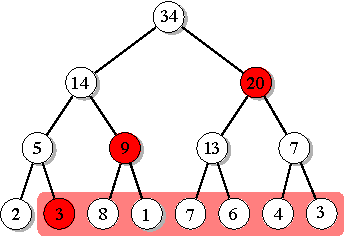
\includegraphics[width=0.5\linewidth]{images/dyadic-ranges}
  \caption{A hierarchy of dyadic ranges. The leaves are the ranges of length $2^0$, while the root corresponds to the single range of length $2^3$. Each level of the tree can be seen as a CM sketch table. To estimate $\sum_{k=2}^8F[k]$, the range $[2,8]$ is decomposed into dyadic ranges $[2,2], [3,4], [5,8]$. Each node contains the sum of the values stored in its children. Red nodes are queried and their sum is returned. Adapted from \cite{Cormode11}.}
    \label{figure:dyadic-ranges}
\end{figure}

  \appendix
\section{Hogwarts}

The Hogwarts School\footnote{\url{http://didawiki.cli.di.unipi.it/lib/exe/fetch.php/magistraleinformatica/alg2/algo2_16/hogwarts.pdf}}
is modeled as a graph $G=(V, E)$ where $V$ is the set of castle's rooms and $E \subseteq V \times V$
is the set of the stairs.
Each stair is labelled with the time of appearance and disappearance, and can be
walked in both directions, therefore the graph is undirected.
The goal is to find, if possible, the minimum amount of time required to go from
the first to the last room.

\subsection{Solution 1: Preprocessing-then-Dijkstra}

Dijkstra is able to find the shortest path in a graph with non-negative weights
on its edges.
Our main idea is to create a Dijkstra compatible graph through a \textsc{normalize}
function, then apply Dijkstra to it in order to find the shortest path.
The core of the preprocessing is the \textsc{normalize} function which computes traversal
times between nodes at a given time \emph{time}:

\begin{algorithmic}[1]
  \Function{normalize}{$from$, $to$, $time$}:
    \State $t \gets \infty$
    \If{$start[v'] \leq t < end[v']$}  \Comment{No waiting time}
      \State $t \gets t + 1$
    \ElsIf{$t < start[v']$}            \Comment{Waiting time}
      \State $t \gets start[v'] + 1$
    \Else
      \State $t \gets \infty$          \Comment{Available time already expired}
    \EndIf
      \State \Return{$t$}
    \EndFunction
\end{algorithmic}

The normalize function is then applied to a node traversal:

\subsubsection{Pseudo-code}

\begin{algorithmic}[1]
  \State create vertex set $Q$ of unvisited nodes\;
  \State create vertexes set $E'$ of edges weight\;
  \State $time \gets 0$                   \Comment{Initial time for traversal}
  \State $edges \gets$ \Call{stairs\_of}{0}\;      \Comment{Get incoming/outgoing edges
   of the source node}
  \Function{process}{$node$, $time$}
    \If{$edge \in visited\_edges$}
      \State \Return{}
    \EndIf

    \State $traversal\_time \gets \infty$
    \ForAll{$neighbor \in neighbors\_of\_node$}
      \State $traversal\_time \gets$ \Call{traversal\_time}{$node$, $neighbor$, $time$}
      \State $E'[0][node] \gets traversal\_time$   \Comment{$E'[i][j]$ holds the
                                                        weight/traversal}
      \State \Comment{time for the stair between $i$ and $j$}

      \ForAll{$new\_neighbor \in neighbors\_of\_neighbor$}
        \State \Call{normalize}{$neighbor$, $new\_neighbor$, $traversal\_time$}
      \EndFor
    \EndFor
    \If{\Call{dijkstra}{$V, E'$} = $\infty$}
    	\State \Return{-1}
    \Else
      \State \Return{$t$}
    \EndIf
  \EndFunction
\end{algorithmic}

\begin{framed}
  \noindent
  \textbf{Computational cost}: $\Theta(n^{2})$ if the vertex set in \textsc{dijkstra} is implemented
  as an array. $O(|E|+|V|\log |V|)$ with Fibonacci heap.
\end{framed}

\subsection{Solution 2: HogwartsDijkstra}

\begin{algorithmic}[1]
  \Function{HogwartsDijkstra}{$G$}:
  \State create vertex set $Q$ of unvisited nodes
  \ForAll{vertex $v \in V$}      \Comment{initialization}
      \State $time[v] \gets \infty$  \Comment{unknown time from source to v}
      \State add $v$ to $Q$          \Comment{all nodes initially in Q}
  \EndFor
  \State $time[0] \gets 0$ \Comment{time from source to source}
  \While{$Q\ne \emptyset$}
      \State $u \gets x \in Q$ with $\min \{time[x]\}$
      \State remove $u$ from $Q$
      \ForAll{neighbor $v$ of $u$}:
          \If{$time[u] \leq appear[v]$}
              \State $alt \gets appear[v] + 1$ \Comment{wait the appearance of
                                                                    the stair}
          \ElsIf{$time[u] < disappear[v]$}
              \State $alt \gets time[u] + 1$       \Comment{use the stair}
          \Else
              \State $alt \gets \infty$            \Comment{the stair has
                                                        already disappeared}
          \EndIf
          \If{$alt < time[v]$}
              \State $time[v] \gets alt$           \Comment{a quicker path to
                                                            $v$ has been found}
          \EndIf
      \EndFor
  \EndWhile
  \State \Return{$time[|N|-1]$}
  \EndFunction
\end{algorithmic}

\begin{framed}
  \noindent
  \textbf{Computational cost}. See the previous section.
\end{framed}

\subsection{Solution 3: BFS-like traversal}

\begin{algorithmic}[1]
  \Function{reach}{$N$, $M$, $A[]$, $B[]$, $appear[]$, $disappear[]$}
      \For{$i=0$ to $M-1$}
          \State $edges\_[A[i]].push\_back(make\_pair(i, B[i]))$
          \State $edges\_[B[i]].push\_back(make\_pair(i, A[i]))$
      \EndFor
      \For{$i=0$ to $N-1$}
          \State $done\_[i] \gets false$
          \State $distance\_[i] \gets \infty$
      \EndFor
      \State $reached\_[0].push\_back(0)$
    \State $distance\_[0] \gets 0$
    \For{$t=0$ to $MAX\_TIME$}
      \ForAll{$v \in reached\_[t]$}
          \If{not $done\_[v]$}
          \ForAll{$edge \in edges\_[v]$}
            \State $staircase \gets edge.first$
            \State $neighbor \gets edge.second$
            \State $time \gets \max(distance_[v], appear[staircase])+1$
            \If{not $done\_[neighbor]$ \\ \hfill and $distance\_[v] < disappear[staircase]$ \\ \hfill and  $time < distance\_[neighbor]$}
              \State $distance\_[neighbor] \gets time$
              \State $reached\_[time].push\_back(neighbor)$
            \EndIf
          \EndFor
        \State $done\_[v] \gets true$
          \EndIf
      \EndFor
    \EndFor
    \State \Return{$(distance\_[N-1] = \infty) ? -1 : distance\_[N-1]$}
  \EndFunction
\end{algorithmic}

\begin{framed}
  \noindent
  \textbf{Computational cost}: $O(m + MAX\_TIME)$.
\end{framed}


\section{Paletta}

Paletta ordering\footnote{\url{http://didawiki.cli.di.unipi.it/lib/exe/fetch.php/magistraleinformatica/alg2/algo2_16/paletta.pdf}}
is a peculiar ordering technique: given a 3-tuple of elements, paletta takes the
central element as pivot and swaps the two elements right before and next to it.
To make an example:
$$(3, 2, 1) \xrightarrow{paletta} (1, 2, 3)$$
We now want to develop an algorithm to order any array through paletta ordering
with the minimal number of swaps.
You should see as not every array can be ordered (e.g. [1, 3, 2]).

\vspace{0.5cm}
\paragraph{Solution.}
We should note that the following properties hold:
\begin{enumerate}
    \item Every element can be a pivot, but the first and the last one, as they
    have respectively no elements before and after them.
    \item Every element can be swapped as many times as necessary, but only with
    elements of the same 2-remainder (numbers in even positions can only be
    swapped with numbers in even positions, the same holds for odd indexes).
    More formally, if $n$ is the size of the array $A$ we want to sort,
    $i,j \in [1, n - 2]$, $A[i]$ can be swapped with $A[j]$ if and only if $i \equiv j \pmod{2}$.
    \item The least number of swaps does not backtrack any element.
    Formally, let \emph{k} be the minimal number of swaps applied to an array,
    backtracks included. By hypothesis, \emph{k} is minimal, but at least \emph{m},
    $m > 0$ backtrack swaps have been operated, therefore we found a
    $k' = k - m: k' < k$, a new minimal number of swaps: contradiction.
\end{enumerate}

Given item 2, we can split our array in two, even and odd numbers, and order
them counting the swaps.
In our example we'll use \emph{mergesort}, as it runs in $O(n\log n)$, does
backtrack elements, and is very well-known.
Clearly, given an array, a swap happens when an element is pushed back, pulling
the one between its new position and the old one ahead: we can map this behaviour
in the merge routine of mergesort: the array merged is able to push back elements
from its right pointer to the new array, moving them back of $(m - i) + (j - m)$ positions,
where \emph{m} is the dimension of the current two sub-arrays to merge.
Provided that our edited version of mergesort ran successfully on both the
even-index and odd-index, we now need to verify if by merging them we obtain an
ordered array.
Intuitively, the merged array will start with the first element of the even-index
arrays, followed by the first of the odd-index array, followed by the second of
the even-index array, and so on.
To check for these elements is pretty trivial and can be done in linear time.
Follows the pseudo-code for the edited version and \textsc{snake\_check} function:

\begin{algorithmic}[1]
  \Function{merge\_with\_paletta}{$left$, $right$, $k$}:
    \State \dots                        \Comment{merge instructions}
    \If{$right > left$}
      \State $paletta\_count \gets paletta\_count + 1$
      \State \dots
      \EndIf
    \EndFunction
\end{algorithmic}

\begin{algorithmic}[1]
  \Function{snake\_check}{}
    \State $even, odd \gets 0$
    \For{;$even, odd < N;even = even + 1, odd = odd + 1$}
      \If{$a[even] > a[odd]$}
        \State \Return{$-1$}\;
      \EndIf
    \EndFor
    \State \Return{$paletta\_count$}\;
    \EndFunction
\end{algorithmic}

\begin{framed}
  \noindent
  \textbf{Computational cost}: $\Theta(n\log n)$.
\end{framed}


\end{document}
